\documentclass[tikz, border=10pt]{standalone}
\usepackage{tikz}
\usetikzlibrary{shapes, shadows, calc, positioning, arrows.meta}

% Define colors
\definecolor{GeoskanBlue}{RGB}{0, 89, 166}
\definecolor{GeoskanOrange}{RGB}{255, 100, 0}
\definecolor{GeoskanBlack}{RGB}{30, 30, 30}
\definecolor{GeoskanSilver}{RGB}{200, 200, 200}
\definecolor{GeoskanGuard}{RGB}{220, 230, 240} % Light transparent blueish for guards

\begin{document}
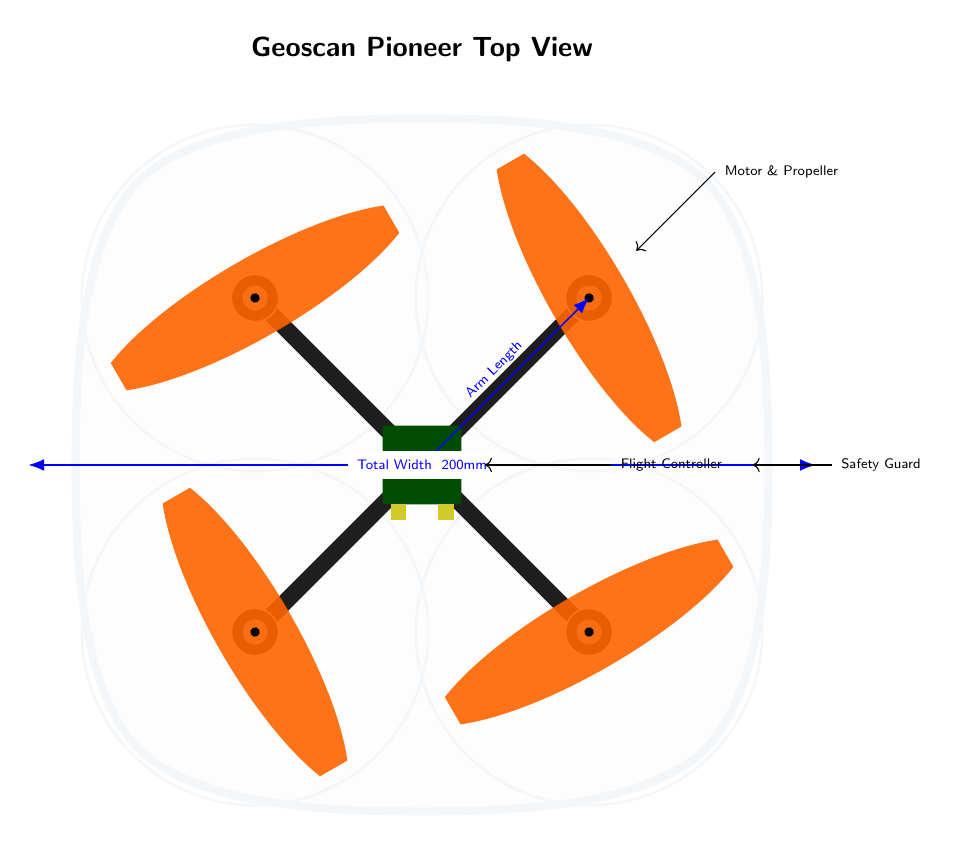
\begin{tikzpicture}[scale=2]

    % Grid (Optional for technical view, can be commented out)
    %\draw[help lines, step=0.5, gray!20] (-3,-3) grid (3,3);

    % --- Define drone geometry ---
    \def\armLength{1.5}
    \def\propRadius{1.0}
    \def\motorRadius{0.15}
    \def\centerSize{0.6}

    % --- Protection Guard (Bottom Layer) ---
    % Semi-transparent simplified guard shape
    \begin{scope}[transparency group, opacity=0.3]
        \draw[line width=3pt, color=GeoskanGuard, fill=GeoskanGuard!20] 
        plot [smooth cycle, tension=0.6] coordinates {
            (2.2, 0) (1.8, 1.8) (0, 2.2) (-1.8, 1.8) 
            (-2.2, 0) (-1.8, -1.8) (0, -2.2) (1.8, -1.8)
        };
        % Inner cutouts for propellers
        \foreach \angle in {45, 135, 225, 315} {
            \draw[line width=1pt, color=GeoskanGuard] (\angle:\armLength) circle (\propRadius + 0.1);
        }
    \end{scope}

    % --- Frame (PCB) ---
    \node[fill=GeoskanBlack, rounded corners=2pt, minimum size=\centerSize cm, inner sep=0pt] (center) at (0,0) {};
    
    % Arms
    \foreach \angle in {45, 135, 225, 315} {
        \draw[line width=6pt, color=GeoskanBlack, line cap=round] (0,0) -- (\angle:\armLength);
        % Motor Mounts
        \fill[GeoskanBlack] (\angle:\armLength) circle (\motorRadius);
        \draw[line width=0.5pt, color=white] (\angle:\armLength) circle (\motorRadius); % Outline
    }

    % --- Electronics (Center) ---
    \fill[green!30!black, rounded corners=1pt] (-0.25, -0.25) rectangle (0.25, 0.25); % Flight Controller
    \fill[yellow!80!black] (-0.2, -0.35) rectangle (-0.1, -0.25); % Connector
    \fill[yellow!80!black] (0.1, -0.35) rectangle (0.2, -0.25); % Connector
    \node[scale=0.3, text=white, font=\sffamily\bfseries] at (0,0) {FC};
    
    % --- Propellers ---
    % Style 1: Spinning disk effect (optional) or static blades
    \foreach \angle/\propAngle in {45/30, 135/-60, 225/30, 315/-60} {
        \begin{scope}[shift={(\angle:\armLength)}, rotate=\propAngle]
            % Hub
            \fill[GeoskanSilver] (0,0) circle (0.08);
            % Blades
            \fill[GeoskanOrange, opacity=0.9] (-0.1, -1.0) .. controls (-0.3, -0.5) and (-0.3, 0.5) .. (-0.1, 1.0) -- 
                                 (0.1, 1.0) .. controls (0.3, 0.5) and (0.3, -0.5) .. (0.1, -1.0) -- cycle;
            % Propeller Hub detail
            \fill[black] (0,0) circle (0.03);
        \end{scope}
    }

    % --- Technical Dimensions ---
    \draw[{Latex[length=2mm]}-{Latex[length=2mm]}, line width=0.5pt, blue] (0,0) -- node[midway, above, sloped, font=\tiny\sffamily] {Arm Length} (45:\armLength);
    \draw[{Latex[length=2mm]}-{Latex[length=2mm]}, line width=0.5pt, blue] (-2.5, 0) -- node[midway, fill=white, font=\tiny\sffamily] {Total Width ~200mm} (2.5, 0);

    % --- Labels ---
    \node[font=\sffamily\bfseries, anchor=south] at (0, 2.5) {Geoscan Pioneer Top View};
    \draw[<-] (45:\armLength) ++(0.3, 0.3) -- ++(0.5, 0.5) node[right, font=\tiny\sffamily] {Motor \& Propeller};
    \draw[<-] (0,0) ++(0.4, 0) -- ++(0.8, 0) node[right, font=\tiny\sffamily] {Flight Controller};
    \draw[<-] (2.1, 0) -- ++(0.5, 0) node[right, font=\tiny\sffamily] {Safety Guard};

\end{tikzpicture}
\end{document}
